\begin{mainquestion}{csoutputswing}{Output Swing and Linearity in a Common-Source Amplifier}

\questionpoints This problem will look at different ways to increase the linearity of a transistor amplifier. The first part sets up the normal amplifier and reviews the way we measure the amplifier non-linearity (which was derived in the lecture notes). The next parts look at different ways to improve the amplifier linearity.  
\\
\\
\\
For this problem, we will assume a square law transistor where:
\[\mu C_{ox}=\kappa'=200\frac{\mu A}{V^2},\ \ \ \  I_{DS}= \frac{1}{2}\kappa'\frac{W}{L} V_{OV}^2,\ \ \ V_{DD}=5V,\ \ \ V_{th}=0.7V\] and the min $L=0.2\mu m.$ In all of the problems we will maintain the same gain of the amplifier.
\\
\\
\\
\\
Let the small-signal be \( v_{in} \).  The linear small-signal approximation predicts:

\[
i_{ds}^{lin} = g_m v_{in} = \frac{2 I_{DS,Q}}{V_{OV}}v_{in}
\]
\\
\\
while the true current variation is the total current minus the current at the bias point:

\[
i_{ds}^{true} = \frac{1}{2}\kappa'\frac{W}{L}(V_{OV}+v_{in})^2 - I_{DS,Q}
\]

\begin{figure}[h]
\centering
\begin{circuitikz}[american, arrowmos]

% -------- Common Source Amplifier --------
\draw
(0,0) node[ground]{}
(0,2) node[nmos] (M1) {}
(M1.S) -- (0,0)

(M1.D) to[R,l=$R_D$] (0,4) -- (0,4.6) node[above]{$V_{DD}$}

(M1.G) -- (-2,2) node[left]{$V_{IN}$}

(M1.D) -- ++(2,0) node[right]{$V_{OUT}$};

\node at (0,-1) {Common-Source Amplifier};

\end{circuitikz}
\end{figure}

%-----------------------------------
\qnewpage

% =========================================================
\begin{partquestion}{widthforgain}
{If $R_D=10k\Omega$, what width transistor is needed to create a gain of 10 amplifier?  Please make the output voltage at the bias point $V_{DD}/2$, and give both the voltage at the gate terminal of the transistor and $V_{OV}$ at the bias point (the DC operating point).}

\begin{answer}[3in]
We want the output bias point to be

\[
V_{OUT,Q} = \frac{V_{DD}}{2} = 2.5V
\]

The drain current at the bias point is determined by the drop across $R_D$:

\[
I_{D,Q} = \frac{V_{DD}-V_{OUT,Q}}{R_D}
       = \frac{5-2.5}{10k\Omega}
       = 0.25\,mA
\]

The gain of a common–source amplifier is

\[
A_v \approx -g_m R_D
\]

For a gain magnitude of 10,

\[
g_m = \frac{10}{R_D}
     = \frac{10}{10k\Omega}
     = 1\,mS
\]

Using

\[
g_m = \frac{2I_D}{V_{OV}}
\]

\[
V_{OV} = \frac{2I_D}{g_m}
       = \frac{2(0.25\,mA)}{1\,mS}
       = 0.5V
\]

Now solve for the transistor size:

\[
I_D = \frac{1}{2}\kappa' \frac{W}{L} V_{OV}^2
\]

\[
\frac{W}{L}
=
\frac{2I_D}{\kappa' V_{OV}^2}
=
\frac{2(0.25\,mA)}
{(200\,\mu A/V^2)(0.5)^2}
=10
\]

Since $L=0.2\mu m$,

\[
W = 10L = 2\,\mu m
\]

The gate voltage is

\[
V_G = V_{TH} + V_{OV} = V_{TH}+0.5V
\]

\textbf{Final results}

\[
I_D = 0.25\,mA
\]

\[
V_{OV} = 0.5V
\]

\[
\frac{W}{L}=10 \quad\Rightarrow\quad W=2\mu m
\]

\[
V_G = V_{TH}+0.5V = 0.7V + 0.5V = 1.2V
\]
\end{answer}

\end{partquestion}

% =========================================================
\begin{partquestion}{nonlinearity}
{We are interested in looking at the non-linearity of the amplifier you designed in part a). While it might seem logical to compute the output voltage for a given input voltage (which works great in this example), in later examples that will be more difficult.  Instead, we will work backward: given an output voltage, we will compute the input voltage needed to create that output.  Since the output voltage depends on the drain current, we can use the drain current to find the input voltage.
\\
\\
Find the input voltage, $v_{in}$ needed to get $\alpha V_{DD}$ at the output, for both the linear small signal model and the quadratic model. Plot the input (y axis) vs. $\alpha$ (x-axis).  You should find that the difference between these two curves is less than 10\% when $\alpha$ is roughly between .3 and .7.}

\begin{answer}[3.5in]
Let the output voltage be

\[
V_{OUT} = \alpha V_{DD}
\]

The drain current through the load resistor is

\[
I_D = \frac{V_{DD}-V_{OUT}}{R_D}
\]

\[
I_D = \frac{(1-\alpha)V_{DD}}{R_D}
\]

Substituting $V_{DD}=5V$ and $R_D=10k\Omega$,

\[
I_D = \frac{5(1-\alpha)}{10k}
     =0.5(1-\alpha)\,mA
\]

The incremental drain current is

\[
i_d = I_D - I_{D,Q}
\]

\[
i_d = 0.5(1-\alpha)-0.25
\]

\[
i_d = 0.25-0.5\alpha \quad (mA)
\]

\textbf{Linear small–signal model}

\[
i_d^{lin}=g_m v_{in}
\]

Since $g_m=1mS$,

\[
v_{in}^{lin}=\frac{i_d}{g_m}
\]

\[
v_{in}^{lin}=0.25-0.5\alpha
\]

\textbf{Quadratic transistor model}

From the square-law relation,

\[
\frac{i_d}{I_{D,Q}}
=
\left(\frac{V_{OV}+v_{in}}{V_{OV}}\right)^2
- 1
\]

Since

\[
\frac{i_d}{I_{D,Q}}
=
\frac{0.25-0.5\alpha}{0.25}
=
1-2\alpha = \left(\frac{V_{OV}+v_{in}}{V_{OV}}\right)^2
- 1
\]

We can now easily solve for $v_{in}$
\[2-2\alpha = \left(\frac{V_{OV}+v_{in}}{V_{OV}}\right)^2
\quad \implies V_{OV}+v_{in}= V_{OV}\sqrt{2-2\alpha}
\]

\[
v_{in}=V_{OV}\left(\sqrt{2-2\alpha }-1\right)\]

Since $V_{OV}=0.5V$,

\[
v_{in}^{true}
=
0.5(1-\sqrt{2-2\alpha})
\]

The two curves agree best near the bias point ($\alpha=0.5$) and begin to diverge near the edges of the output swing. At \(\alpha = .7\), the small signal model gives\(v_{in}^{lin}=0.25-0.5\alpha=.1V\) where the quadratic model gives \(0.5(1-\sqrt{2-2\alpha})=.11V\)

\begin{center}
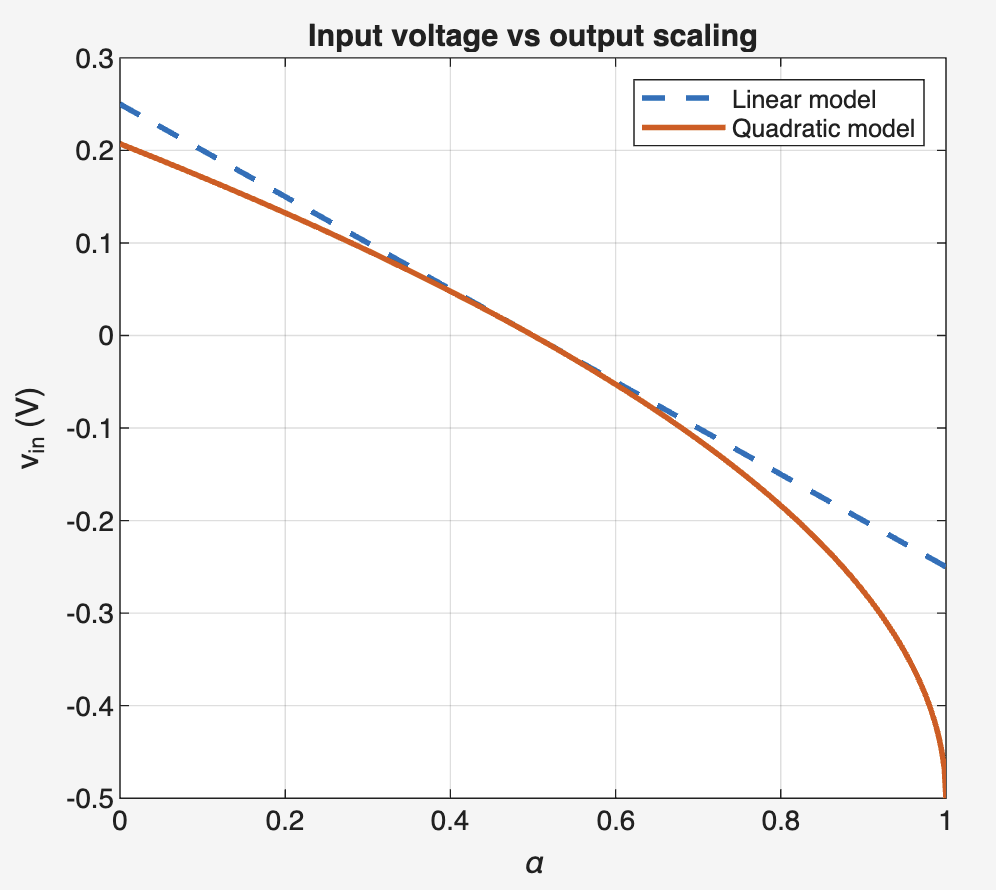
\includegraphics[width=0.8\linewidth]{q1b.png}
\end{center}
\end{answer}

%-----------------------------------

\begin{figure}[h]
\centering
\begin{circuitikz}[american, arrowmos]

% -------- Source Degeneration Amplifier --------
\draw
(6,0) node[ground]{}
to[R,l=$R_S$] (6,1.5)

(6,3.5) node[nmos] (M2) {}

(M2.S) -- (6,1.5)

(M2.D) to[R,l=$R_D$] (6,5.5) -- (6,6.1) node[above]{$V_{DD}$}

(M2.G) -- (4,3.5) node[left]{$V_{IN}$}

(M2.D) -- ++(2,0) node[right]{$V_{OUT}$};

\node at (6,-1) {With Source Degeneration};

\end{circuitikz}
\end{figure}
\pagebreak
%-----------------------------------
\end{partquestion}

% =========================================================
\begin{partquestion}{addrs}
{We will try to improve the linearity by adding a resistor, $R_S$, between the source and ground. This resistor will effect the gain of the transistor, so we first need to figure out that effect. Let's use the same transistor and $R_D$ as in part a), and we'll make $R_S=500 \Omega$. Since the source voltage is no longer at ground, $v_{GS}$ is no longer equal to $V_{IN}$. So to keep $v_{GS}$ constant (and the transistor bias current the same, which keeps the output voltage at $V_{DD}/2$) we need to raise the $V_{IN}$ bias voltage.  What is this new bias voltage, and what is the gain of this new amplifier (at the new bias point)?}

\begin{answer}[2.5in]
The bias current must remain the same so the output voltage stays at $V_{DD}/2$.

Thus

\[
I_D = 0.25\,mA
\]

The voltage across the source resistor is

\[
V_S = I_D R_S
\]

\[
V_S = (0.25\,mA)(500\Omega)
\]

\[
V_S = 0.125V
\]

Since $v_{GS}$ must remain unchanged, the gate voltage must increase by this amount.

Original gate voltage:

\[
V_G = V_{TH}+0.5V
\]

New gate voltage:

\[
V_G = V_{TH}+0.5+0.125
\]

\[
V_G = V_{TH}+0.625V = 0.7V + 0.625V = 1.325V
\]

To find the new gain, we account for the source degeneration resistor. The gain of a common-source amplifier with source degeneration is:

\[
A_v = \frac{-g_m R_D}{1 + g_m R_S}
\]

Using $g_m = 1\,mS$ (from part a), $R_D = 10\,k\Omega$, and $R_S = 500\,\Omega$:

\[
A_v = \frac{-(1\,mS)(10\,k\Omega)}{1 + (1\,mS)(500\,\Omega)}
\]

\[
A_v = \frac{-10}{1 + 0.5} = \frac{-10}{1.5} \approx -6.67
\]
\end{answer}

\qnewpage
\end{partquestion}

% =========================================================
\begin{partquestion}{degeneratedgain}
{Computing the gain of this new configuration is difficult because as you change $V_{IN}$, both the gate and source voltages change! In this circuit, setting the output current, and then measuring what $V_{IN}$ is needed makes the task much easier.  Once you know the output current, you should also know the voltage across $R_S$, and should be able to compute $v_{GS}$ to give you $V_{IN}$. 

Show that, for this transistor with a source resistor, the effective $g_m'=\frac{1}{R_S+1/g_{m_o}}$, where $g_{m_o}$ is the transistor's $g_m$.}

\begin{answer}[3in]
Let $g_{m0}$ be the intrinsic transistor transconductance.

Small-signal current:

\[
i_d = g_{m0} v_{gs}
\]

The source voltage is

\[
v_s = i_d R_S
\]

Since

\[
v_{gs} = v_{in} - v_s
\]

\[
v_{gs} = v_{in} - i_d R_S
\]

Substitute $i_d=g_{m0}v_{gs}$:

\[
v_{gs} = v_{in} - g_{m0}v_{gs}R_S
\]

\[
v_{gs}(1+g_{m0}R_S)=v_{in}
\]

\[
v_{gs}=\frac{v_{in}}{1+g_{m0}R_S}
\]

Now

\[
i_d=g_{m0}v_{gs}
\]

\[
i_d=
\frac{g_{m0}}{1+g_{m0}R_S}v_{in}
\]

Thus the effective transconductance is

\[
g_m'=\frac{i_d}{v_{in}}
=
\frac{g_{m0}}{1+g_{m0}R_S}
\]

Rearranging,

\[
g_m'=\frac{1}{R_S+\frac{1}{g_{m0}}}
\]

Using this newly derived effective transconductance, we can also compute the gain of the amplifier to confirm our result from the previous section:

\[
A_v = -g_m' R_D
\]

\[
A_v = - \left( \frac{1}{R_S + \frac{1}{g_{m0}}} \right) R_D
\]

Substituting our known values ($R_S = 500\,\Omega$, $g_{m0} = 1\,mS$, $R_D = 10\,k\Omega$):

\[
A_v = - \left( \frac{1}{500 + 1000} \right) 10000
\]

\[
A_v = -\frac{10000}{1500} \approx -6.67
\]
\end{answer}

%-----------------------------------
\end{partquestion}

% =========================================================
\begin{partquestion}{redesign}
{We now want to change the amplifier design to get a gain of 10 with the $500\Omega$ source resistor. Given the effective transconductance is now $g_m'=\frac{1}{R_S+1/g_{m_o}}$, find the new transistor width that is needed to make $g_m'=\frac{10}{R_D}$.  With this new design, compute the required input voltage as a function of the output voltage.  Is the linearity better? What range of output is within a 10\% error now?}

\begin{answer}[2.5in]
We want the gain magnitude to remain 10:

\[
|A_v| = g_m' R_D
\]

Thus

\[
g_m' = \frac{10}{R_D}
\]

\[
g_m' = \frac{10}{10k\Omega}
=1mS
\]

Using the effective transconductance expression

\[
g_m'=\frac{1}{R_S+1/g_{m0}}
\]

\[
1mS = \frac{1}{500 + 1/g_{m0}}
\]

\[
500 + \frac{1}{g_{m0}} = 1000
\]

\[
g_{m0} = 2mS
\]

Now compute the new overdrive voltage:

\[
V_{OV}=\frac{2I_D}{g_{m0}}
\]

\[
V_{OV}=\frac{2(0.25mA)}{2mS}
\]

\[
V_{OV}=0.25V
\]

Now solve for the new transistor size:

\[
I_D=\frac12\kappa' \frac WL V_{OV}^2
\]

\[
\frac{W}{L}
=
\frac{2I_D}{\kappa'V_{OV}^2}
=
\frac{2(0.25mA)}
{(200\mu A/V^2)(0.25)^2}
=40
\]

Since \(L=0.2\mu m\),

\[
W = 40L = 8\mu m
\]

\textbf{Input voltage vs output voltage}

Using the same approach as in part b), we know that:
\[
i_d = 0.25mA -0.5\alpha  \quad (mA)
\]

The source voltage is

\[
v_S = i_d R_S= 125mV(1-2 \alpha)
\]

Like in part b) we use the current to find the needed \(v_{gs}\), but since the source isn't at ground, this needs to be added to \(v_s\) to get the full input voltage. The gate voltage required to produce this current is found using the normalized drain current:

\[\frac{i_{ds}}{I_{DS}}=1-2\alpha =\left(\frac{V_{OV}+v_{gs}}{V_{OV}}\right)^2
- 1\]

\[v_{gs}=V_{OV}\left(\sqrt{2-2\alpha }-1\right)\]
Since $V_{OV}=.25V$ now:
\[v_{gs}=0.25V\left(\sqrt{2-2\alpha }-1\right)\]

So the required input voltage is:
\[v_{in}=0.25V\left(\sqrt{2-2\alpha }-1\right)+ 0.125V (1-2 \alpha)\]

\textbf{Linearity}
Notice that even though the gain is the same, the size of the $\sqrt{}$ term is now have as large, so the distortion is about 1/2 of what it was before. 
Numerical comparison of the linear and quadratic models shows that the
amplifier remains within about 10\% error up to approximately

\[
V_{out} \approx 0.78V_{DD}
\]

which is larger than the original amplifier's linear range
(approximately \(0.3V_{DD}\)–\(0.7V_{DD}\)).

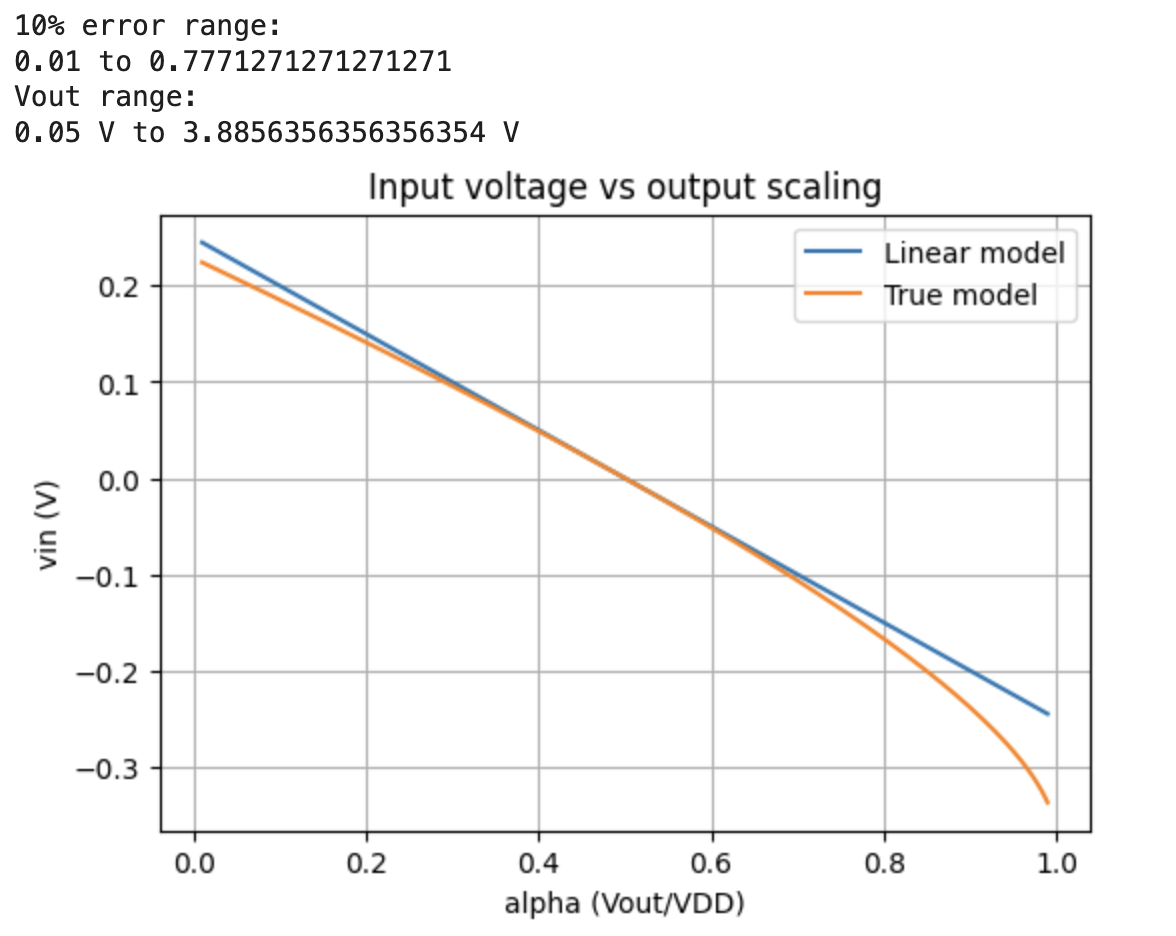
\includegraphics[width=0.8\linewidth]{q1e.png}

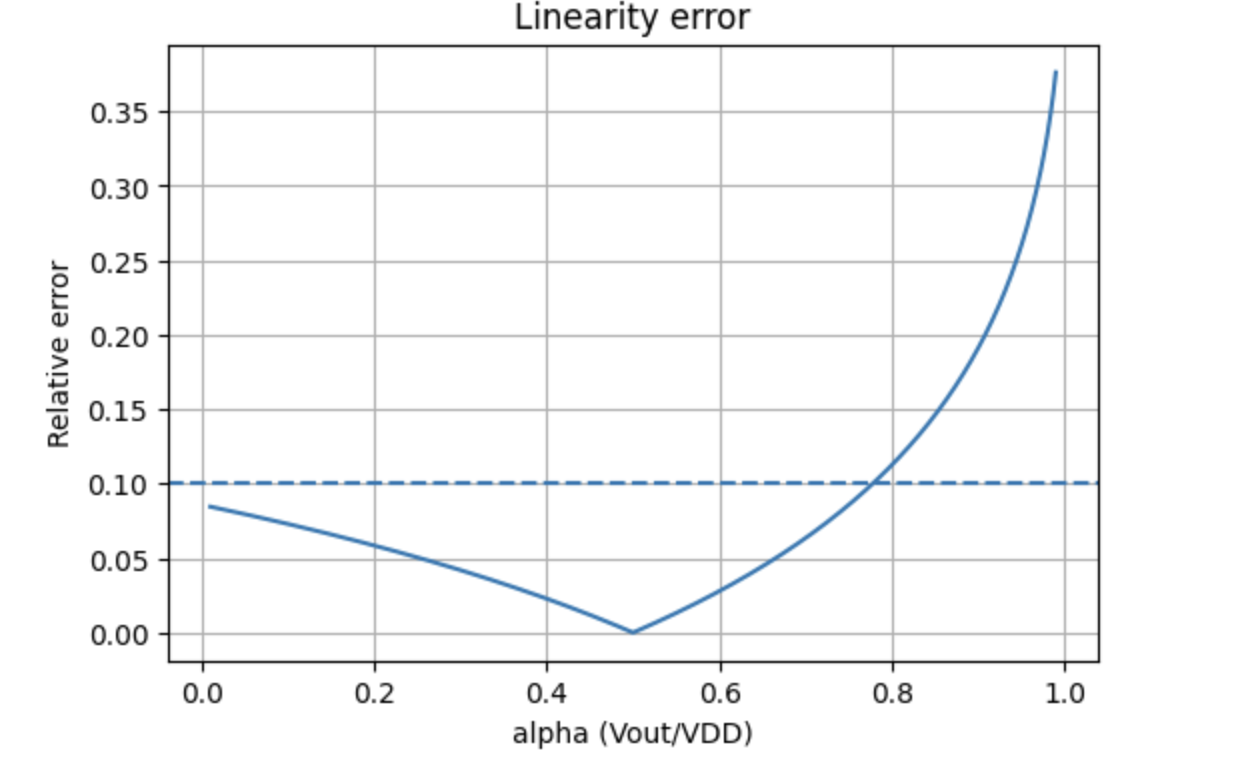
\includegraphics[width=0.8\linewidth]{q1e2.png}
\end{answer}

\pagebreak
%-----------------------------------
\end{partquestion}

% =========================================================
\begin{partquestion}{currentvariation}
{The problem with our transistor amplifier is that the current through the transistor is quadratic with voltage. So as you move through the full current range, you must see non-linearity.  If you want to really reduce the non-linearity of the amplifier, you need to make the output swing over the entire voltage range while only needing to change the current by a fraction of its full range.  While this might seem impossible, it is quite easy to do!  Just add a current source in parallel with the resistor. This current source can be built using a pMOS transistor in saturation!
\begin{figure}[h]
\centering
\begin{circuitikz}[american, arrowmos]

% -------- Common Source Amplifier --------
\draw
(0,0) node[ground]{}
(0,2) node[nmos] (M1) {}
(M1.S) -- (0,0)

(M1.D) to[R,l=$R_D$] (0,4) -- (0,4.6) node[above]{$V_{DD}$}

(M1.G) -- (-2,2) node[left]{$V_{IN}$}

(M1.D) -- ++(2,0) node[right]{$V_{OUT}$}

(1,4.6) node[above]{$V_{DD}$} to[I] (1,2.75);

\end{circuitikz}
\end{figure}

Let's make this current $0.6 \cdot I_{DS}$.  Notice that the nMOS transistor now needs to sink all this current before the output voltage will start to fall. Using the transistor design from part a), and using the same input bias point, resize the load resistor $R_D$ so the output at the bias point is still $V_{DD}/2$. What is the new gain? What is the non-linearity now?}

\begin{answer}[3.5in]
The added current source supplies

\[
I_{CS}=0.6I_{D,Q}
\]

\[
I_{CS}=0.6(0.25mA)=0.15mA
\]

At the bias point the NMOS still draws $0.25mA$, so the resistor carries

\[
I_R = I_D - I_{CS}
\]

\[
I_R = 0.25 - 0.15
\]

\[
I_R = 0.10mA
\]

To keep the output at $V_{DD}/2=2.5V$,

\[
R_D = \frac{2.5V}{0.10mA}
\]

\[
R_D = 25k\Omega
\]

The new gain is

\[
A_v = -g_m R_D
\]

\[
A_v = -(1mS)(25k)
\]

\[
A_v = -25
\]

For a swing from 1V to 4V ($20\%-80\%$ of full scale, and roughly the range where the transistors will remain saturated) the transistor current only swings from $0.68 I_{DS}, .4V$ to $1.32I_{DS}, 1V$. Therefore the required variation in $v_{GS}$ is smaller, which significantly improves the linearity of the amplifier. For this range of current swing the distortion we computed in part b) was less than 10\%.  
\end{answer}

\textit{(Actually once we have added a current source, it probably makes sense to make it roughly $I_{DS}$ and remove the resistor all together.  The $R_o$ of the transistor and the current source will provide an output resistance, and you can get very high gains.  Just make sure you use some feedback on the biasing, otherwise you will miss the high-gain region!)}
\end{partquestion}

\end{mainquestion}
